\chapter[Contextualização]{Contextualização}

\section{Problema}

		Tirar chopp é uma arte.  Não há muito que se discutir, ao se conversar com apreciadores (\textit{sommeliers}) do mesmo,  eles hão de concordar que isso  deve ser feito com paixão, dedicação  e técnica, para que se obtenha o máximo de qualidade. Requisitos que muitas vezes não são cumpridos por aqueles que servem o chopp como emprego.
        
        Dado o custo  envolvido com o trabalho de garçons, demora no atendimento, falta de praticidade, ausência de padronização na tiragem do chopp e problemas de controle de temperatura, os quais contribuem para a desvalorização do produto, prejudicam o seu consumo, bem como encarecem o mesmo, deseja-se minimizar as ocorrências do que  foi citado. 


\section{Estado da Arte}

No mundo inteiro, a cada dia, mais e mais pessoas se deixam seduzir pelo insuperável sabor das bebidas fermentadas, como a cerveja, e particularmente o chope. Assim sendo esse permite a existência de um mercado que estimule a criatividade de muitos empreendedores.

Hodiernamente a bebida é um atrativo para casas noturnas e eventos que ao longo dos anos ganhou vários apreciadores, possuindo inclusive eventos voltados apenas para os degustadores da bebida. 

Um exemplo é o sistema MyTapp de uma \textit{startup} de Florianópolis.  O sistema faz a venda de chopp ao estilo \textit{self-service}, no qual os usuários compram créditos para uso da máquina e podem colocar somente a quantidade que consumirem. Esse sistema favorece novatos no consumo de chopp que têm a oportunidade de serem cobrados somente pelo que consumirem, podendo provar diversos tipos de chopp. A figura abaixo mostra o uso desse sistema.

Outro exemplo de equipamento de ponta é uma chopeira  que se encontra no Japão. Ela é capaz de servir de forma automática os copos e localiza-se no Aeroporto Internacional de Kansai (KIX) em Osaka. A foto abaixo encontra-se na imagem a seguir.

\section{Objetivos}

\subsubsection{Gerais}

    Construir uma maquina de chopp que realiza a a tiragem de chopp de forma automatizada, seguindo o paradigma de uma Vending Machine.
    
\subsubsection{Objetivos Específicos}

\begin{itemize}
\item{Servir automaticamente o chopp.}

\item{Comprovar autenticação da compra previamente efetuada.}

\item{Efetivar a compra  de forma online.}

\item{Inclinar o copo, de acordo com os padrões de tiragem de chopp.
Controlar a quantidade de espuma no copo (colarinho) de acordo com a escolha do usuário e padrões predefinidos.}

\item{Selecionar a quantidade de chopp a ser servida, de acordo com padrões prévios.}

\item{Fornecer energia de forma suplementar em casos emergenciais.
Permitir a escolha entre dois tipos de chopp.}

\end{itemize}


\section{Escopo}

Trata-se de uma solução de venda remota para compra de chopp no cartão, servindo com preferências predefinidas (colarinho, quantidade e tipo), realizando a venda de forma autônoma otimizando a tiragem do chopp. Essa solução é obtida a partir de um sistema que possui alimentação redundante de energia por um certo período de tempo, fazendo parte de um sistema para controle da quantidade e das vendas de chopp. O escopo não engloba: (i) O congelamento do chopp; (ii) A produção do chopp ou de seu gás; (iii) a venda de drinks, cerveja, refrigerantes e alimentos; (iv) o pagamento via dinheiro em espécie; (v) uma máquina outdoor; (vi) a troca automática do chopp (feito manualmente); (vii) o reuso do copo, assumindo que os copos que serão consumidos serão reusados.

\section{Estrutura Analítica do Projeto}

A seguir, na Figura \ref{eap} se encontra a Estrutura Analítica do Projeto (EAP), ilustrando todos os entregáveis que agrega valor ao produto. A EAP está dividida pela correspondente Engenharia responsável.

\begin{figure}[!hb]
    \centering
    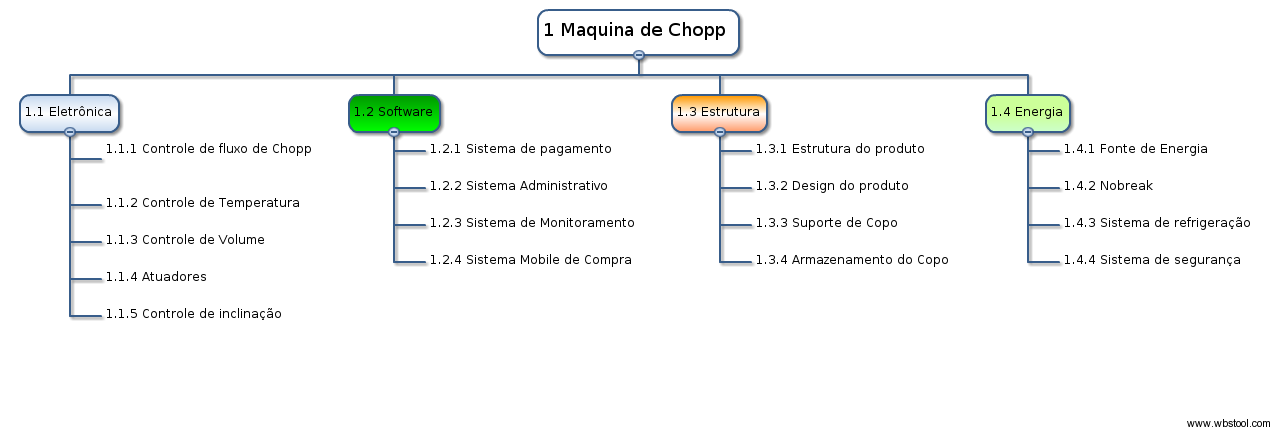
\includegraphics[scale=0.4]{figuras/eap.png}
    \caption{Estrutura Analítica do Projeto.}
    \label{eap}
\end{figure}